\documentclass{article}

\usepackage{tikz}
\usepackage{amsfonts}
\usepackage{amssymb}
\usepackage{mathtools}
\usepackage{nameref}
\usepackage{xcolor}

\usepackage[english]{babel}
\usepackage[autostyle]{csquotes}
\MakeOuterQuote{"}

\usepackage[backend=biber,style=numeric]{biblatex}
\addbibresource{CoC_EliDupree_Edition.bib}

\title{The Calculus of Constructions, EliDupree Edition}
\author{Eli Dupree}
\date{\today}

\DeclareMathSymbol{\mlq}{\mathord}{operators}{``}
\DeclareMathSymbol{\mrq}{\mathord}{operators}{`'}

\newcommand{\Prop}{\mathbb{P}}
\newcommand{\istype}{\ \mathrm{type}}
\newcommand{\usage}{\mathcal{V}}
\newcommand{\usageKnown}[2]{{\usage_{\mlq\hspace{-0.06em}#2\hspace{-0.06em}\mrq}^{:#1}}}
\newcommand{\presep}{\hspace{1.8em}}
\newcommand{\subst}[3]{#1^{[{#2}{/}{#3}]}}
\newcommand{\subty}[1]{#1^*}
\newcommand{\bindvariable}{\bigstar}
\newcommand{\bindnotthis}{\circ}
\newcommand{\emptybindingslike}[1]{\varnothing #1}
\newcommand{\betaeq}{\cong}
\newcommand{\betared}[1]{\overset{#1}{\rightarrow}}
\newcommand{\anywhat}{\ell}

\begin{document}
  \maketitle
  
  \section{Introduction}
  
  This document describes the Calculus of Constructions (CoC), using the specific definitions that I (Eli Dupree) refined from the original definitions.
  
  Section \ref{fundamentals} (\textit{\nameref{fundamentals}}) gives a formal definition of CoC.
  
  Section \ref{structure} (\textit{\nameref{structure}}), which is currently much shorter, describes some of the structure that occurs based on those definitions.
  
  I hope to expand this document with more details (such as how to use CoC in practice), but I also hope to define those details by \emph{actually building them}; we'll see what form that takes in practice.
  

  \section{Fundamentals}\label{fundamentals}
  \subsection{Formulas}

  The Calculus of Constructions (CoC) is a system of formulas. The following context-free grammar shows the six elementary "formula constructors" – ways to build a formula, sometimes from smaller formulas ($F$):

  \[ F \rightarrow \Prop \mid \usage \mid \usageKnown{F}{F} \mid \lambda b:F,F \mid \forall b:F,F \mid (F F) \]
  
  By combining these constructors into larger formulas, you can express all of computation and mathematics. Our definitions are mainly concerned with judging which of these formulas are \textbf{types}, and which other formulas are \textbf{members} of those types. Anywhere you see the symbol $:$, as in $v : T$, it means a claim that something is a member of the type $T$.

  Here is an informal description of each formula constructor:

  $\Prop$ (read as "Prop") is the \emph{type of all ordinary types}. It's called "Prop" because the ordinary types can represent \emph{propositions} (although they can represent many other things as well).
  
  $\lambda b:T,v$ ("a lambda") is a \emph{function} which maps a single parameter, of type $T$, to the formula $v$ (after the value of the parameter is substituted into $v$). We call $T$ the \textbf{parameter type}, and $v$ the \textbf{body} or the \textbf{return value}.
  
  $\forall b:T,U$ ("a forall", read as "for all $b$ in $T$, $U$") is the \emph{type} of a lambda. We call these types "foralls" because of the way that types can represent propositions: The members of a type are the proofs of a proposition, and a proposition with no proofs (an empty type) is a false proposition\footnote{A fan of Gödel might ask: "What about propositions that are true but unprovable?" Well, we are free to define "true" to mean "provable within CoC". We are speaking of \emph{constructive} truth, which is a slightly stronger claim than truth in classical logic. Like all theories, CoC must be incomplete, but the form of that incompleteness is just that there are some propositions $P$ where neither $P$ nor $\neg P$ is provable.}. If the proposition $U$ is true for all members of the type $T$, then you can write a lambda that maps any member of $T$ to a member of $U$, and that lambda will be a member (a proof) of $\forall b:T,U$. As with lambdas, we call $T$ the \textbf{parameter type}, and $U$ the \textbf{body} or the \textbf{return type} (because it will be the type of the return value of such a lambda).
  
  $\usage$ is a \emph{variable usage}, which may appear inside the body of a lambda or forall, as a location to substitute in the value of the parameter. $\usageKnown{T}{i}$ is the same, but with an explicit definition of its type and variable-identity.
  
  $(f v)$ ("an apply") is a \emph{function application} – the kind that would be written $f(v)$ in the notation of usual math or programming. CoC is based on the lambda calculus, where this is written as $f v$.
  
  Before we can make these definitions formal, we must take a couple of detours.
  
  

  \subsection{Variable identities}

  You may note that I haven't defined the $b$ in $(\lambda b:T,v)$. If you know lambda calculus, you're expecting $b$ to be a variable name. But due to some definitional inconveniences\footnote{Using variable names requires you to define "alpha-conversions" and "contexts", and to make substitutions allow renaming bindings. Our formulation allows us to dispense with these complications – at the price of a somewhat-smaller amount of different complications.}, we use a different (yet equivalent) definition. $b$ is a \textbf{binding tree}, with the following grammar:

  \[b \rightarrow \bindvariable \mid \bindnotthis \mid (b b) \]

  This requires some explanation. In the usual lambda calculus, you may write something like

  \[ \lambda x : \mathrm{Number}, ((\mathrm{plus}\ 2)\ x) \]

  to mean the function which maps any number to the same number plus 2. This formula actually uses the symbol $x$ in two different ways. The first occurrence of $x$ is a \textbf{binding}, introducing a new variable that will henceforth be called "$x$". The second occurrence of $x$ is a \textbf{usage}, saying to substitute in the value that was previously named "$x$". Similarly, if you want a function with multiple parameters, you may write
  
  \[ \lambda x : \mathrm{Number}, \lambda y : \mathrm{Number}, ((\mathrm{plus}\ x)\ y) \]

  In our definitions, every \textbf{usage} is the formula $\usage$, so the body becomes
  
  \[ \lambda x : \mathrm{Number}, \lambda y : \mathrm{Number}, ((\mathrm{plus}\ \usage)\ \usage) \]
  
  So how do you tell that it means $x + y$, rather than $x + x$ or $y + y$? The answer is that our \textbf{bindings}, $x$ and $y$ themselves, will tell you this. The full expansion is this:
  
  \[ \lambda (\bindnotthis((\bindnotthis \bindvariable) \bindnotthis)) : \mathrm{Number}, \lambda ((\bindnotthis \bindnotthis) \bindvariable) : \mathrm{Number}, ((\mathrm{plus}\ \usage)\ \usage) \]
  
  This is best visualized as a tree, where each lambda's binding-tree is the \emph{same shape} as the whole body of that lambda:
  
  \begin{center}
  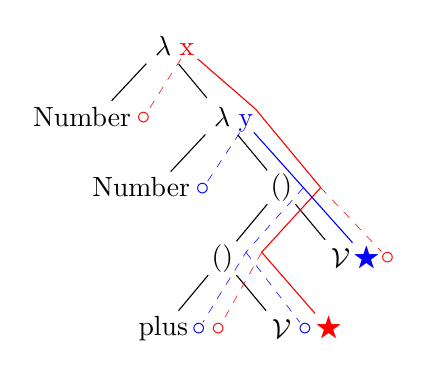
\begin{tikzpicture}
    \draw (0,0) node[inner sep=3pt](lx){$\lambda$}[level distance = 0.9cm]
      child {node[xshift=-0.8em,inner sep=2pt]{Number} [child anchor=28]}
      child {node[inner sep=3pt](ly){$\lambda$}
        child {node[xshift=-0.8em,inner sep=2pt]{Number} [child anchor=28]}
        child {node[inner sep=1pt]{()}
          child {node[inner sep=1pt]{()}
            child {node[inner sep=2pt]{plus}}
            child {node[inner sep=3pt]{$\usage$}}
          }
          child {node[inner sep=3pt]{$\usage$}}
        }
      };
    \path(lx) +(0.3,-0.05) node[red,inner sep=1pt](x){x}
      (lx-1) +(0.78,-0.02) node[red,inner sep=0pt](x01){$\bindnotthis$}
      (ly) +(0.42,0.02) node(x0){}
      (ly-2)+(0.5,-0.08) node(x1){}
      (ly-2-2)+(0.6,0) node[red,inner sep=0pt](x2){$\bindnotthis$}
      (ly-2-1)+(0.5,0) node(x3){}
      (ly-2-1-1)+(0.7,0) node[red,inner sep=0pt](x4){$\bindnotthis$}
      (ly-2-1-2)+(0.6,0) node[red,inner sep=1pt](x5){$\bindvariable$};
    \path(ly) +(0.3,-0.09) node[blue,inner sep=0pt](y){y}
      (ly-1) +(0.78,-0.02) node[blue,inner sep=0pt](y01){$\bindnotthis$}
      (ly-2)+(0.28,-0.08) node(y1){}
      (ly-2-2)+(0.33,0) node[blue,inner sep=1pt](y2){$\bindvariable$}
      (ly-2-1)+(0.3,0) node(y3){}
      (ly-2-1-1)+(0.45,0) node[blue,inner sep=0pt](y4){$\bindnotthis$}
      (ly-2-1-2)+(0.3,0) node[blue,inner sep=0pt](y5){$\bindnotthis$};
    
    \draw[red](x) -- (x0.mid) -- (x1.mid) -- (x3.mid) -- (x5);
    \draw[red,very thin,dashed]
      (x) -- (x01)
      (x1.mid) -- (x2)
      (x3.mid) -- (x4);
    \draw[blue](y) -- (y1.mid) -- (y2);
    \draw[blue,very thin,dashed]
      (y) -- (y01)
      (y1.mid) -- (y3.mid) -- (y4)
      (y3.mid) -- (y5);
    
%    \draw(ly-2-1) +(0.3,0) -- (y);
%    \draw (0.2cm,0) node[above]{$x$}[level distance = 1cm]
%      child {node{$\bindnotthis$}}
%      child {
%        child {node{$\bindnotthis$}}
%        child {
%          child {
%            child {node{$\bindnotthis$}}
%            child {node{$\bindvariable$}}
%          }
%          child {node{$\bindnotthis$}}
%        }
%      };
  \end{tikzpicture}
  \end{center}
  
  In this example, the red tree rooted at $x$ selects the first $\usage$ (by marking it with $\color{red}\bindvariable$), and the blue tree rooted at $y$ selects the second $\usage$ (by marking it with $\color{blue}\bindvariable$). If we wanted to express $x + x$, we could make the first binding tree have a $\color{red}\bindvariable$ at both locations, and the second have only $\color{blue}\bindnotthis$s.
  
  Observe that it is straightforward to convert between the "variable names" form and the "binding trees" form:
  \begin{itemize}
    \item If you are given valid variable names, you can write binding trees that place $\bindvariable$ at the locations of the usages with the same name.
    \item If you are given valid binding trees, you can give each binding a name, and write that name on each usage where the tree had a $\bindvariable$.
  \end{itemize}
  
  Thus, when giving example formulas, we may sometimes write them using the "variable names" form, even though the formal definition uses the "binding trees" form. To avoid ambiguity, we reserve the letters $b,c,d$ for binding trees, and $x,y,z$ for variable names.
  
  There is one remaining complication. When we write the typing rules for formulas like $\lambda b:T,v$, we will sometimes have to consider the sub-formula $v$ in isolation. But from $v$'s perspective, $b$ is no longer available to help clarify which usages inside $v$ refer to which bindings. This is the purpose of the formula-constructor $\usageKnown{T}{i}$, a usage that has explicit knowledge of its type $T$ and identity $i$. ($i$ is technically another formula, but its only purpose is to be distinct from the value of $i$ for any other variable that was not bound at the same site.) When we want to consider $v$ in isolation, we will \emph{replace} each $\usage$ with $\usageKnown{T}{i}$, at any location where $b$ had a $\bindvariable$.\\
  
  Finally, for a formula $F$ to be valid, it must be \textbf{well-bound}, meaning:
  \begin{itemize}
    \item For every occurrence of $\usage$ in $F$, there is exactly one binding tree that places a $\bindvariable$ at that location. All other trees place a $\bindnotthis$ there.
    \item For every occurrence of $\Prop$ or $\usageKnown{T}{i}$ in $F$, \emph{all} trees place a $\bindnotthis$ there.
  \end{itemize}
  
  Any formula that is not well-bound is \textbf{ill-bound}. Ill-bound formulas are not very interesting\footnote{They cannot have types or be members of types. Moreover, this will occur naturally as a result of the typing rules, without any explicit rules to enforce it.}, so we generally work only with well-bound formulas. But sub-formulas may be technically ill-bound when viewed in isolation, and we will \emph{sometimes} view them this way.
  
  Having defined binding trees, we may now rigorously define \emph{variable substitution}.
  
  
  
  \subsection{Substitution}
  
  The whole point of variables is to be able to substitute them for other values. In algebra, we say $x^2 + x + 2$, knowing that we can later replace $x$ with \emph{any} number and have the formula retain its meaning. In CoC, we want to do much the same thing, just using lambdas instead. Instead of $x$, we have the binding tree; instead of "number", we have the parameter type.
  
  To achieve this, we'll introduce some formal notation. In the following rules, the symbols $F,G,H,T,U,f,v,w$ mean "any formula", and the symbols $b,c,d,e,f$ mean "any binding tree". Technically, by "any", we mean \emph{universal quantification, scoped outside the statement}. That is, if a statement includes two copies of the same symbol (say, $T$), then the statement is true for all possible values of $T$, but only when the two usages of $T$ represent the \emph{same} formula.
  
  We now define the following concepts:
  
  \begin{itemize}
  \item $\subst{F}{b}{v}$ ("formula subsitution") means the formula you get when you start with $F$ and insert one copy of $v$ at the location of each $\bindvariable$ in $b$.
  \item $\subst{c}{b}{d}$ ("binding tree subsitution") is the same thing for binding trees, starting with $c$ and inserting a copy of the \emph{tree} $d$ at the location of each $\bindvariable$ in $b$.
  \item $\emptybindingslike{v}$ ("empty bindings shaped like") means an empty binding tree shaped like the formula $v$.\footnote{The need to define $\emptybindingslike{v}$ is one of the few complications added by the "binding tree" form. However, if we used variable names, we would instead have to allow variable-renaming here, which is not any simpler.}
  \end{itemize}
  
  
  
  Formally,  
  \[\emptybindingslike{\usage} = \bindnotthis\]
  \[\emptybindingslike{\Prop} = \bindnotthis\]
  \[\emptybindingslike{\usageKnown{T}{i}} = \bindnotthis\]
  \[\emptybindingslike{(\lambda b:T,v)} = (\emptybindingslike{T}\ \emptybindingslike{v})\]
  \[\emptybindingslike{(\forall b:T,U)} = (\emptybindingslike{T}\ \emptybindingslike{U})\]
  \[\emptybindingslike{(f v)} = (\emptybindingslike{f}\ \emptybindingslike{v})\]
    
  \[\subst{\bindnotthis}{\bindvariable}{d} = d\]
  \[\subst{\bindnotthis}{\bindnotthis}{d} = \bindnotthis\]
  \[\subst{\bindvariable}{\bindnotthis}{d} = \bindvariable\]
  \[\subst{(bc)}{(de)}{f} = (\subst{b}{d}{f}\ \subst{c}{e}{f})\]
  
  \[\subst{\usage}{\bindvariable}{v} = v\]
  \[\subst{\Prop}{\bindnotthis}{v} = \Prop\]
  \[\subst{\usageKnown{T}{i}}{\bindnotthis}{v} = \usageKnown{T}{i}\]
  \[\subst{(\lambda b:T,w)}{(cd)}{v} = \lambda \subst{b}{d}{\emptybindingslike{v}}:\subst{T}{c}{v},\subst{w}{d}{v}\]
  \[\subst{(\forall b:T,U)}{(cd)}{v} = \forall \subst{b}{d}{\emptybindingslike{v}}:\subst{T}{c}{v},\subst{U}{d}{v}\]
  \[\subst{(f w)}{(cd)}{v} = (\subst{f}{c}{v}\ \subst{w}{d}{v})\]

The main reason we define substitution is for \emph{function application}. If you have a function $f =(\lambda b:T,w)$, then you want $(f v)$ to be equivalent to $\subst{w}{b}{v}$.

When we say "equivalent", we can't mean that they are the \emph{same formula} (because they are not). But we would like to say that they are two different formulas that refer to the \emph{same object}. This notion is formalized in the concept of \textbf{fold-equivalence}, written $\betaeq$, which we will now build out of several pieces.

The transformation $(f v) \rightarrow \subst{w}{b}{v}$ is called \textbf{lambda unfolding}. We would like to be able to unfold any lambda within a formula. That is, if $(f v)$ appears as a sub-formula of a larger formula – say, $(g (f v))$ – then we would also like to say $(g (f v)) \rightarrow (g(\subst{w}{b}{v}))$.

For this, we need\footnote{The typical definitions don't need this, and indeed, this is the one place where the "binding tree" form adds more complexity than it removes.} a notion of \textbf{what-lambda} is being unfolded, with the following grammar:

\[\anywhat \rightarrow \mathcal{L}\anywhat \mid \mathcal{R}\anywhat \mid b\]
  
  This represents a path starting at the root of the formula, with a choice of "left" or "right" at each step, ending in the binding-tree specifying which usages are being replaced.

  We now introduce a few more notations:
  
  \begin{itemize}
  \item The symbol $\anywhat$ means "any what-lambda" (using the same meaning of "any" as before).
  \item $F \betared{\anywhat} G$ means "the formula $F$ becomes $G$ when you unfold $\anywhat$".
  \item $b \betared{\anywhat} c$ means "the binding-tree $b$ becomes $c$ when you unfold $\anywhat$".
  \item $\frac{premises}{conclusions}$ means that if all the premises above the line are true, then all the conclusions below the line are also true. (If the premises are $\varnothing$, then the conclusions are true unconditionally.)
  \end{itemize}
  
  Formally, the single-step unfoldings are:
  
\[ \frac{\varnothing}{((\lambda b:T,w)v) \betared{b} \subst{w}{b}{v} \presep ((c d) e) \betared{b} \subst{d}{b}{e}} \]
\[ \frac{b \betared{\anywhat} c}{(b d) \betared{\mathcal{L}\anywhat} (c d) \presep (d b)\betared{\mathcal{R}\anywhat} (d c)} \]
\[ \frac{F \betared{\anywhat} G}{(F H) \betared{\mathcal{L}\anywhat} (G H) \presep (H F) \betared{\mathcal{R}\anywhat} (H G) \presep (\lambda b:F,v) \betared{\mathcal{L}\anywhat} (\lambda b:G,v) \presep (\forall b:F,U) \betared{\mathcal{L}\anywhat} (\forall b:G,U)} \]
\[ \frac{F \betared{\anywhat} G \presep b \betared{\anywhat} c}{(\lambda b:T,F) \betared{\mathcal{R}\anywhat} (\lambda c:T,G) \presep (\forall b:T,F) \betared{\mathcal{R}\anywhat} (\forall c:T,G)} \]

Of these rules, the most interesting one is the last, which requires that both the body formula and the bindings be unfolded at the same lambda. This is necessary because, when any outer lambda had $\bindvariable$s \emph{inside $v$}, those $\bindvariable$s need to be moved/copied to the new location(s) of $v$. 

Having defined single-step unfoldings, we now define fold-equivalence as the smallest equivalence relation that contains them. Intuitively, $F \betaeq G$ if there is a "path" of foldings or unfoldings that converts $F$ to $G$. Formally,

(unfolding is equivalence)
\[ \frac{F \betared{\anywhat} G}{F \betaeq G} \]
(reflexivity\footnote{We don't technically need to assert reflexivity here, because it can be proven from the other rules. But it would be frivolous to leave it out "just because we can".})
\[ \frac{\varnothing}{F \betaeq F} \]
(symmetry)
\[ \frac{F \betaeq G}{G \betaeq F} \]
(transitivity)
\[ \frac{F \betaeq G \presep G \betaeq H}{F \betaeq H} \]
  
  \subsection{Type judgments}
  
  We can now define the substance of CoC: The rules about which formulas are types, and which formulas are members of those types.
  
  \begin{itemize}
  \item "$F\istype$" means "the formula $F$ \textbf{is} a type".
  \item "$F : G$" means "the formula $F$ is a \textbf{member} of the type $G$". (We will make sure this only occurs when the formula $G$ is actually a type.)
  \end{itemize}
  
  Formally,
  
  "Prop is a type":
  \[ \frac{\varnothing}{\Prop\istype} \]  
  
  "Props are types":
  \[ \frac{T : \Prop}{T\istype} \]
  
  "Usages are what they say they are":
  \[ \frac{T\istype}{\usageKnown{T}{i}:T} \]
  
  "Foralls are types":
  \[ \frac{T\istype\presep \subst{U}{b}{\usageKnown{T}{U}}\istype}{(\forall b:T,U)\istype} \]
  
  "Foralls can be Props":
  \[ \frac{T\istype\presep \subst{U}{b}{\usageKnown{T}{U}} : \Prop}{(\forall b:T,U) : \Prop} \]
  
  "Lambdas belong to foralls":
  \[ \frac{\subst{v}{c}{\usageKnown{T}{U\!v}} : \subst{U}{b}{\usageKnown{T}{U\!v}} \presep (\forall b:T,U)\istype}{(\lambda c:T,v) : (\forall b:T,U)} \]
  
  "Applications are the type they'd unfold into":
  \[ \frac{f : (\forall b:T,U) \presep v : T}{(f v) : \subst{U}{b}{v}} \]
  
  "You can fold or unfold types":
  \[ \frac{v : T \presep T \betaeq U \presep U\istype}{v : U} \]
  
  We say that a formula $F$ is a \textbf{value} if it is a member of any type. And a formula is \textbf{well-typed} if it is either a type or a value.
    
  We can now formalize the statement "$F$ and $G$ refer to the same object". An \textbf{object} is an equivalence class of well-typed formulas under $\betaeq$, and any well-typed formula "refers" to the class it belongs to. This makes the statement "$F$ and $G$ refer to the same object" equivalent to "$F \betaeq G$ and both are well-typed".
  
  A few notes on these definitions:
  
  The two rules of foralls are almost identical, and indeed, previous formulations of CoC\cite{coquand1990proof}\cite{rodrigueztype} have expressed them as a single rule, by abstracting over the distinction between "being a type" and "being a member of Prop". However, the two rules have substantially different meanings. "Foralls are types" is the basic definition of the role of foralls. "Foralls can be Props" gives them an additional power, sometimes known as \textbf{impredicativity}: A forall whose parameter type is $\Prop$ can still be a member of $\Prop$ itself, meaning that it quantifies over a category that \emph{includes itself}. This is very mathematically powerful, and only narrowly avoids a paradox of self-reference.
  
  The "You can fold or unfold types" rule can also be read as "Types are objects, not formulas". If $v : T$, then $v$ is also a member of any other formula that represents the same object as $T$.
  
  % TODO: is this actually true?: Although this rule allows a formula to be a member of more than one formula, it's the only rule that does so. Thus, we can say that any formula can only be a member of one \emph{object}.
  % TODO: is this actually true?: also the apply rule means values are objects
  

  \section{Type relationships}\label{structure}
  All well-bound formulas of CoC can be immediately classified into one of the following groups, knowing only the formula constructor and the groups of its immediate sub-formulas.

  \vspace{0.5cm}
  
  \newcommand\toprow{U}
  \newcommand\midrow{Y}
  \newcommand\botrow{D}

  \noindent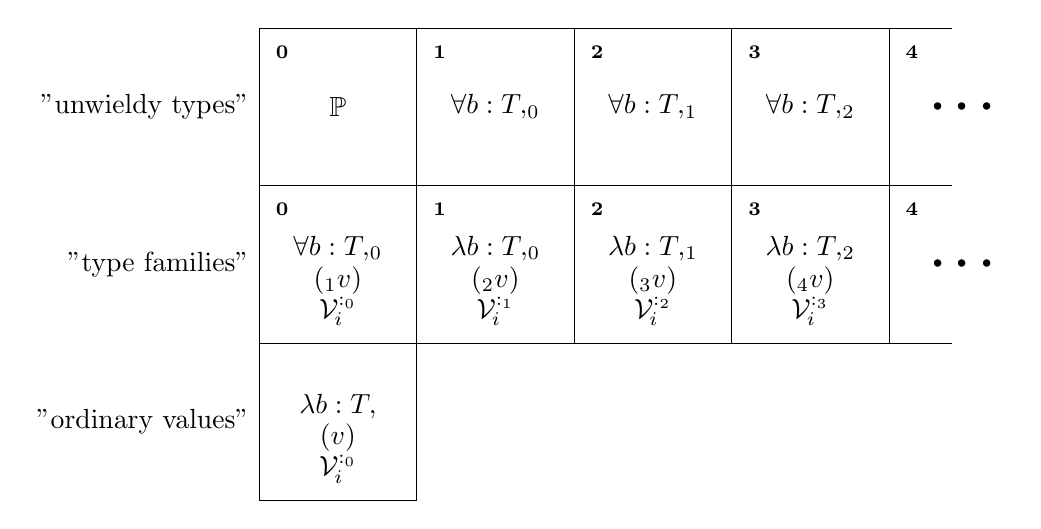
\begin{tikzpicture}
    \pgfsetxvec{\pgfpoint{2cm}{0}}
    \pgfsetyvec{\pgfpoint{0}{-2cm}}

    \draw (0,0.5) node[left]{"unwieldy types"};
    \draw (0,1.5) node[left]{"type families"};
    \draw (0,2.5) node[left]{"ordinary values"};
    \foreach \y in {0,1,2} {
      \draw (0,\y) rectangle (1,\y+1);
      \draw (4,\y) -- (4.4,\y);
    }
    \foreach \y in {0,1} {
      \draw (4.2,\y+0.5) node[right]{{\LARGE \boldmath $\cdots$}};
    }
    \foreach \x in {0,1,2,3,4} {
      \draw (\x+0.15,0.15) node[]{{\boldmath $\toprow_\x$}};
      \draw (\x+0.15,1.15) node[]{{\boldmath $\midrow_\x$}};
    }
    \foreach \x in {0,1,2,3} {
      \draw (\x+0.5,1.8) node[]{$\usageKnown{\toprow_\x}{i}$};
    }
    \draw (0.15,2.15) node[]{{\boldmath $\botrow$}};
    \draw (0.5,0.5) node[]{$\Prop$};
    \draw (0.5,1.4) node[]{$\forall b:T,\midrow_0$};
    \draw (0.5,1.6) node[]{$(\midrow_1 v)$};
    \draw (0.5,2.4) node[]{$\lambda b:T,\botrow$};
    \draw (0.5,2.6) node[]{$(\botrow v)$};
    \draw (0.5,2.8) node[]{$\usageKnown{\midrow_0}{i}$};
    \foreach \l/\x/\r in {0/1/2,1/2/3,2/3/4} {
%      \pgfmathsetmacro{\l}{\x-1};
      \draw (\x,0) rectangle (\x+1,1);
      \draw (\x+0.5,0.5) node[]{$\forall b:T,\toprow_{\l}$};
      \draw (\x,1) rectangle (\x+1,2);
      \draw (\x+0.5,1.4) node[]{$\lambda b:T,\midrow_{\l}$};
      \draw (\x+0.5,1.6) node[]{$(\midrow_{\r} v)$};
    }
  \end{tikzpicture}

  \vspace{0.5cm}

  In the above chart, the literal $T$ can denote any \emph{type}, and $v$ can denote any \emph{value}. The other letters refer to cells; for example, $\midrow_2$ can denote any formula from the cell $\midrow_2$.
  
  % TODO: is this actually correct? (footnote was on "if" below): \footnote{In general, it may be very difficult to determine whether a formula has a type \emph{at all}. But it is easy (again, $O(n)$) to give any formula $V$ a \emph{provisional} type $T$, where if $V$ has any types at all, its types are exactly all the well-typed beta-conversions of $T$. The only difficult part is determining whether function arguments have the correct types.}

  If a formula has a type, that type is in the cell directly above its own. Thus, \emph{values} (formulas that can be members of types) can be in any cell except the top row, and \emph{types} (formulas that can have members) can be in any cell with another cell under it. As such, $\midrow_0$ is the unique cell whose formulas are both types and values.
  
  $\midrow_0$ and $\botrow$ are the easiest to work with. Objects in $\midrow_0$ are called \textbf{ordinary types}, and objects in $\botrow$ are called \textbf{ordinary values}. Sometimes we will also call them, respectively, the \textbf{propositions} and the \textbf{proofs}. Since $\toprow_0$ contains \emph{only} the formula $\Prop$, every ordinary type (proposition) is a member of $\Prop$.
  
  Object in the top row are called \textbf{unwieldy types}. Because they aren't members of any other type, they can't be passed as a parameter values (because parameters must always declare their types), nor returned from lambdas (because a lambda is not well-typed unless its body has a type). The middle row – \emph{members} of unwieldy types – are the \textbf{unwieldy values}. Unwieldy values can freely be passed as parameters, and \emph{can} be returned from lambdas – but a lambda that \emph{returns} an unwieldy value also becomes unwieldy itself. (Note that the ordinary types are also unwieldy values.)
  
  
  
  \printbibliography
\end{document}
